\documentclass[a4j,10pt]{jsarticle}
\usepackage{layout,url,resume}
\usepackage[dvipdfmx]{graphicx}
\pagestyle{empty}

\begin{document}

\title{
RISC-Vの実装と設計
}

\author{
Arch B1 nem
\and
親:tatsu-san
}

\pagestyle{empty}

\begin{abstract}
RISC-Vを実装しようとした。
\end{abstract}

\maketitle

\section{動機}
筆者がCanSatを制作しているサークルに所属していることに起因している。CanSatで用いるマイクロコンピュータを自作したいという希望からFPGAを使用することを考え、ハードウェア記述言語の学習を始めHDLの学習として、RISC-VのRV32Iを設計と実装し、FPGA上で動作させることを目標とした。

\section{実装}
ソースコードはhttps://github.com/NeM-T/cpuにて公開している。

\subsection{開発環境}
\begin{itemize}
\item Vivado 2019.2
\item 言語:SystemVerilog
\item FPGA:Zynq-7010
\end{itemize}

\subsection{実装した命令}
add、sub、or、and、lw、sw、addiを実装した。
残りの命令を実装するより先に論理合成をしようとしてつまってしまった。

\subsection{CPUの構成}
右に構成図を示す。

\begin{figure}[htbp]
    \begin{center}
        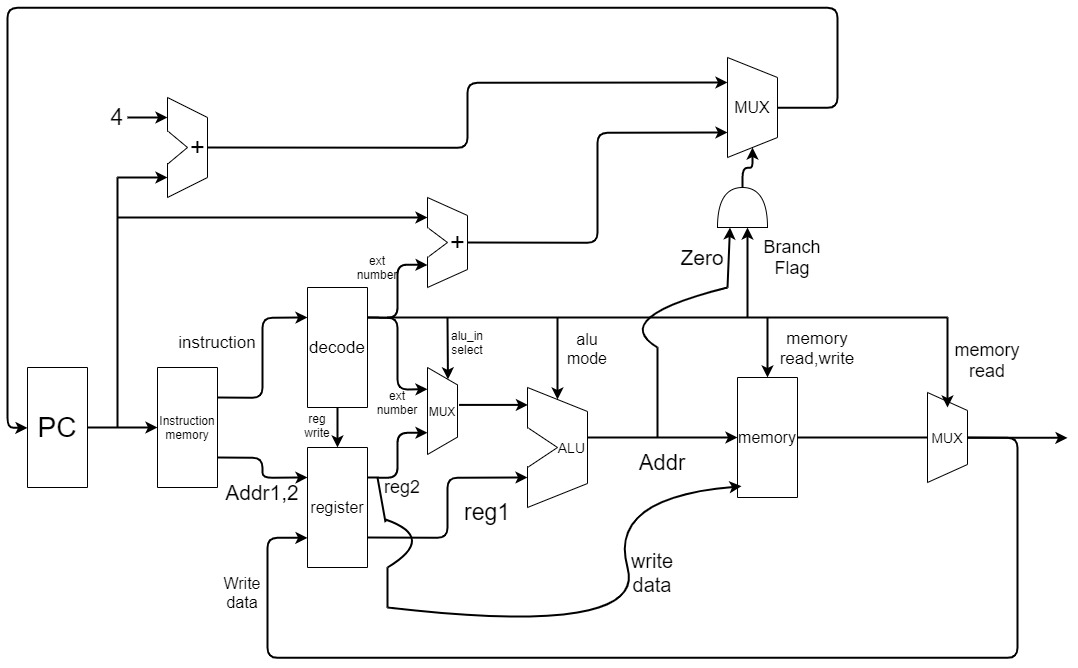
\includegraphics[width=10cm]{./com.jpg}
        \caption{構成}
        \label{sample}
    \end{center}
\end{figure}
 
\subsection{HDLのシミュレーション}
実行した命令は以下のとおりである。

\begin{enumerate}
\item add reg1, reg2, reg1 
\item add reg1, reg2, reg1
\item sub reg1, reg2, reg1  
\item or reg1, reg2, reg3 
\item and reg1, reg2, reg3
\item sw mem1, 2
\item lw mem1, reg1
\item addi reg1, 3, reg1
\end{enumerate}

以下に結果を画像で示す。
\begin{figure}[htbp]
    \begin{center}
        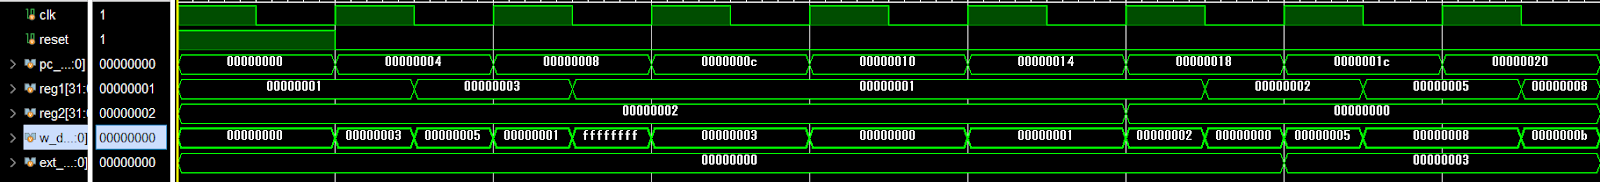
\includegraphics[width=10cm]{./simu.png}
        \caption{シミュレーション結果}
        \label{simu}
    \end{center}
\end{figure}

\subsection{論理合成}
論理合成はできたが、論理合成後のシミュレーションがHDLのみのシミュレーションと違う結果になってしまっている。

\section{今後}
まずは現在のコードを正しく動作できるようにすることを目標にしたい。
その後はRV32Iをすべて実装し、パイプライン化などの高速化の知識を身につけたい。

\end{document}

